\chapter{Ethics and Responsible Disclosure} \label{ethics_chapter}

\section*{Layout}

\begin{enumerate}
    \item Computer Laws
    \item Cyber-ethical dilemmas
    \item Responsible disclosure
\end{enumerate}

\section{Computer Laws}\label{sec:comp_laws}

Israel's computer laws\footnote{Published in \emph{Sefer Hachukkim} 5755 No. 1534, 25 July 1995 p. 366 (P.L. 5754 No. 2278 p. 478).}
are \textit{case-laws} – meaning there are a few written
laws, and a judge would use those along with precedents and personal judgment to
determine whether a person is guilty. This is opposed to
\textit{continental-law}, in which everything is written and proceedings are
executed literally by the book.

\subsection{Definitions}
\begin{enumerate}
    \item "computer material" - software or computer information
    \item "computer" - A device that works with a software to perform arithmetic or logical processing of data and peripherals, with exception to auxiliary computer
    \item "auxiliary computer" - A device that is only able to perform arithmetic processing
    \item "information" - or computer information, is signs, instructions, data or concepts, except for software. the information is expressed via computer language and stored in the computer or any other media or volume.
    \item "output" - any information that is produced or derived via the computer
    \item "computer language" - appropriate expressive form for interpretation, delivery or processing by computer
    \item "software" - A group of instructions expressed in the computer language that can cause a computer to function or to perform an action, and is either embedded or marked with a device or by means of electronic, electromagnetic, electro-optics or any other means, or either united with the computer in some way or separated from it
\end{enumerate}

The laws state which cyber-activities are considered illegal, as follows:
\begin{enumerate}
    \item Unlawfully disrupting or interfering with a computer system
    \item Unlawfully modifying or deleting any material or files from the computer system
    \item Providing false information or false output
    \item Unlawful access, invade or penetrate to a computer system
    \item Unlawful eavesdrop, according to the Wiretap Act 1979 rule
    \item As the above, but in order to commit another offence
    \item Creating, distributing or offering to another person a computer virus (a virus can perform variety of malicious actions, such as removing/changing files, ransomware, backdoor, etc.)
\end{enumerate}

From this we learn that not any crime committed with the aid of a computer
constitutes a cyber-crime; if a computer was used in the process of the crime,
but none of the above computer laws were broken -- for example while
profiteering\footnote{The activity of taking unfair advantage of a situation to make a large profit, 
often by selling goods that are difficult to get at a very high price (Cambridge Business English Dictionary).} 
off an online ticket sale -- the action, while illegal, is not a cyber
crime.


\subsection{Unlawful Disruption or Interfering with a Computer System}

\paragraph{Definition.} Disrupting the normal operation of a computer,
interfering with the use of a computer or deleting of materials saved on a
computer.

Let's observe some examples:
\begin{itemize}
    \item[$\boxtimes$] Performing a DDoS attack on a server
    \item[$\boxtimes$] Infecting a computer with a virus preventing access to
    information saved on it
    \item[$\boxtimes$] Recruiting a computer into a botnet, thus draining its
    resources
    \item[$\square$] Infecting a computer with a program that sends information
    from it to a remote server
    \item[$\square$] Cheating at a single player video game
    \item[$\square$] Installing an unlicensed program
\end{itemize}

All of the above actions are illegal. The first three are violations of the
first section of Israel's computer laws, while the latter three are illegal for
other reasons, since they do not directly prevent/interfere with the victim's
system's functions.

\subsection{False Information or Output}

\paragraph{Definition.} Misinformation; generating, or changing the code of a
program such that it would generate information that is forged or misleading.
Let's observe some examples:
\begin{itemize}
    \item[$\boxtimes$] Sending an email on behalf of someone else without their
    consent
    \item[$\boxtimes$] Changing the code of a grade-calculating program in order
    to change the output grades
    \item[$\boxtimes$] Cheating in an online game to gain an unfair advantage
    \item[$\boxtimes$] Using a \textit{key generator}: a program that forges
    fake software licenses
    \item[$\square$] Recruiting a computer into a botnet
    \item[$\square$] Accessing an email inbox of another user
\end{itemize}

All of the above actions are illegal, but only the first four violate the second
section of Israel's computer laws.

\subsection{Unlawful Access}

\paragraph{Definition.} Virtual trespassing; any action which results in the
perpetrator accessing information to which they do not have access, such as
images, text files, code, etc.

Let's observe some examples:
\begin{itemize}
    \item[$\boxtimes$] Viewing personal information of coffee shop patrons by
    using the same Wi-Fi
    \item[$\boxtimes$] Penetration testing (attempting to find weaknesses) on a
    company's server without its consent
    \item[$\boxtimes$] Using some else's password to access their inbox without
    their consent
    \item[$\square$] Using a program to forge credit card numbers
\end{itemize}

Forging credit card numbers, while illegal, does not fall under this section of
the law; it is constitutes as false information. Note that penetration testing
is a violation of this section of the law even if it is unsuccessful.

\section{Cyber Ethics}\label{sec:cyber_ethics}

We first present two case studies, then proceed to discuss them and cyber ethics
in general.

\subsection{Case Studies}

\paragraph{Stresser.} Two people from Israel ran a DDoS service, known as
Stresser, which performed DDoS attacks on websites for money. They made a large
profit, but were eventually caught, and claimed they were ethical, and there are
occasions where they refused to attack Israeli websites. What were their
motives?

\paragraph{Eternal Blue.} In 2013, the NSA found a vulnerability in
Windows~\cite{CVE-2017-0144} and secretly built a tool called Eternal Blue to
exploit it. At some point, a group of hackers known as the Shadow Brokers stole
security tools from the NSA and offered to sell them on the Dark Net. When
nobody paid, the Shadow Brokers leaked the tools. Microsoft released a patch to
fix the bug a short time later; the patch was prepared in advance after
Microsoft was tipped off by the NSA.

In 2017, a piece of malware known as ``WannaCry" first appeared; it utilized
Eternal Blue to spread quickly through computers on which the security patch
wasn't yet installed, and encrypt the victim's files, then asking for money to
decrypt them\footnote{This is known as ransomware. Recall that this falls under
the first section of the computer laws.}.

\begin{figure}[!ht]
    \centering
    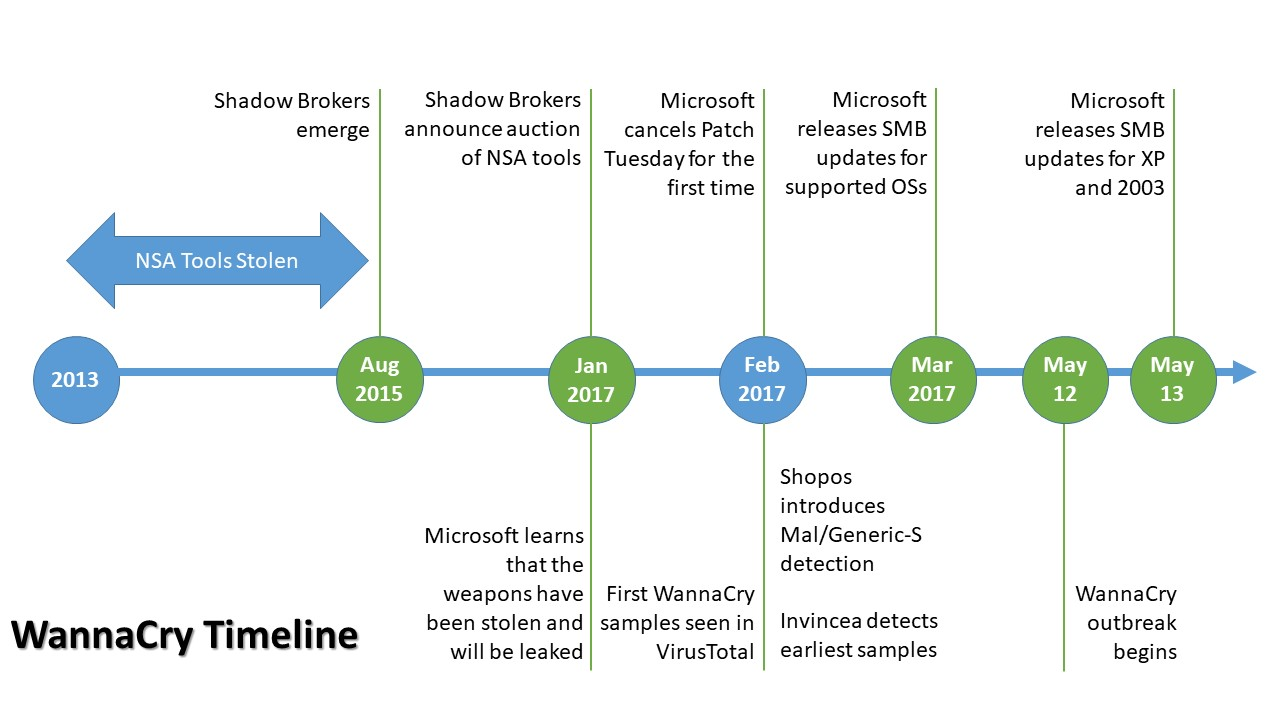
\includegraphics[width=\textwidth]{images/EthernalBlue-WannaCry_Timeline.jpg}
    \caption{EthernalBlue-WannaCry Timeline} \label{fig:wannacry_timeline}
\end{figure}

WannaCry was finally beaten when a malware researcher found it made requests to
an unused control domain, and purchased the domain.\footnote{Malware researchers
often try to purchase control domains in order to gain information on the
behavior of the malware.} As it turned out, purchasing the domain triggered the
destruction of WannaCry, whether by mistake or by design (the domain could have
been designed as a kill-switch).

While WannaCry did not make a lot of money, it had a nasty side-effect on
healthcare systems; medical equipment that got infected could not function
normally, with dangerous, possibly lethal, repercussions.

Suppose a man was killed due to a failure induced by WannaCry; let John be such
a casualty. There are many parties in this story, each holding part of the blame
for John's death:
\begin{itemize}
    \item WannaCry's writers, whose malware caused John's death
    \item Microsoft, whose software was used and trusted by the hospital
    \item The hospital, which relied solely on Microsoft's software without
    providing safety measures of their own
    \item The NSA, who knew about the bug well in advance, but did not perform
    responsible disclosure
    \item The Shadow Brokers, who leaked the NSA's tools to the public, which
    lead to the development of WannaCry
\end{itemize}

\subsection{Discussion}
\paragraph{Ethics.} Ethical behavior is deciding how to act according to one's
moral system. It is mostly instinctive, or composed of a personally devised
code, rather than conforming to a set of rigid universal rules.

\paragraph{The Trolley Problem\cite{foot1967problem}.} Imagine a trolley approaching a fork in the
railway. On the first path lie five people, and on the second only a single
person. The trolley, if its course remains unchanged, will head for the first
path, resulting in the deaths of the five people there. However, you as a
bystander have the option to pull a lever to change the direction of the trolley
to the second path, resulting in the single death of the man there.

\begin{figure}[!ht]
    \centering
    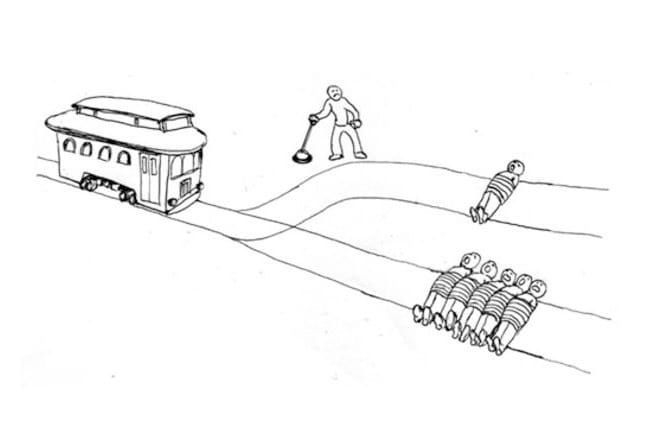
\includegraphics[width=\textwidth]{images/The_Trolley_Problem.jpg}
    \caption{The Trolley Problem} \label{fig:trolley_problem}
\end{figure}

According to the numbers, you should pull the switch to save the five. But in
that case, by sending the trolley toward the single person on the other path,
you are \textit{directly} responsible for his death! So should you avoid getting
involved, thus allowing the deaths of five people instead?

What if one of the people is a close friend? Would that change your answer?

There is another version to this problem, in which there is only a single road
with five people on it. You, along with a very large man, are standing on a
bridge above the road, and you have the option of \textit{pushing} the large man
beside you off the bridge to block the approaching trolley. The stakes are the
same, but in the scenario, in order to save the five you need to actually commit
murder!

\begin{figure}[!ht]
    \centering
    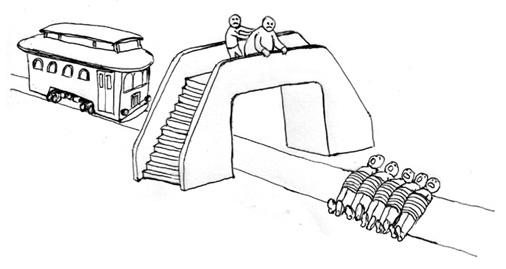
\includegraphics[width=\textwidth]{images/The_Trolley_Problem_Fat_Man.jpg}
    \caption{The Trolley Problem (Fat Man)}
    \label{fig:trolley_problem_fat_man}
\end{figure}

Our ``closeness" to a situation affects on how we judge it by our moral standards.

\paragraph{How to decide.} There are two main theories by which the morality of
an action is judged:
\begin{itemize}
    \item Deontological ethics (Kant\footnote{Immanuel Kant was a German philosopher during the
    Enlightenment era. His contributions have had a profound impact on almost every philosophical movement that followed him.})
    -- what do my rules/morals say about this
    action? (i.e. judge by motives)
    \item Utilitarian ethics (Bentham\footnote{Jeremy Bentham was an English philosopherduring the
    Enlightenment era and a social reformer regarded as the founder of modern utilitarianism.}) -- what are the consequences of this
    action? (i.e. judge by consequences)
\end{itemize}

Consider the cyber setting. If we were to program ethics into an AI (say, an
autonomous car), we would have to use Utilitarian Ethics -- a score system by
which the algorithm could judge what would be the least terrible outcome
according to our moral system.

This presents complications; for example, let's consider a practical
implementation of the Trolley Problem in autonomous cars: Assume a car is
driving on a bridge containing five pedestrians in the middle of the road. If
the car continues on its path, they will all die. However, the car can choose to
veer off the bridge, saving five lives but killing the driver. By utilitarian
considerations, this is the best approach – but who will purchase a car which is
programmed to kill him on certain circumstances?

\paragraph{Cyber crime.} Our brain is ``programmed" to feel distressed when
confronted with an unethical scene; i.e. when we see a scene of a person
committing an unethical act, we feel bad in sympathy with the victim. This is
why it is easier to commit a cyber crime -- we do not see the victim, and do not
sympathize with them. Upholding cyber ethics would mean artificially causing
users to use their judgment when their brains would not.

\section{Responsible Disclosure}
Disclosure is the act of alerting a product vendor to a vulnerability in their
product so that they could patch it. Disclosure is performed by an honest party
(i.e. not a hacker who wishes to exploit the vulnerability) with the intention
of increasing the security of the product. There is a question of exactly when
and how to perform this disclosure.

An exploit is considered as \textit{zero day} when the vendor is unaware of the
vulnerability it exploits (meaning it is known only to a few, and unknown to the
general public - i.e. it has not been disclosed).

\Cref{fig:vulnerability_timeline} describes a timeline of a vulnerability from the moment
it is found to the moment its patch is deployed.

\begin{figure}[!ht]
    \centering
    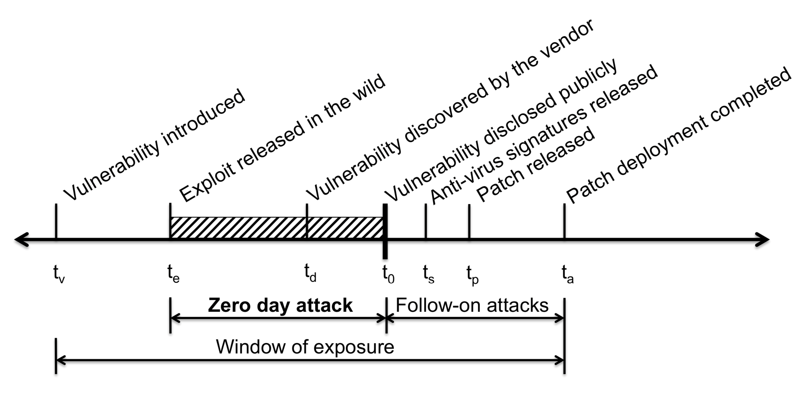
\includegraphics[width=\textwidth]{images/Vulnerability_Timeline.PNG}
    \caption{Timeline of a vulnerability} \label{fig:vulnerability_timeline}
\end{figure}

Symantec, the company founding Nortron\footnote{Norton is an anti-virus.}, had a
lot of data regarding vulnerabilities and exploits, and used it to research the
matter. \Cref{fig:disclosure_research_findings} shows their results.

\begin{figure}[!ht]
    \centering
    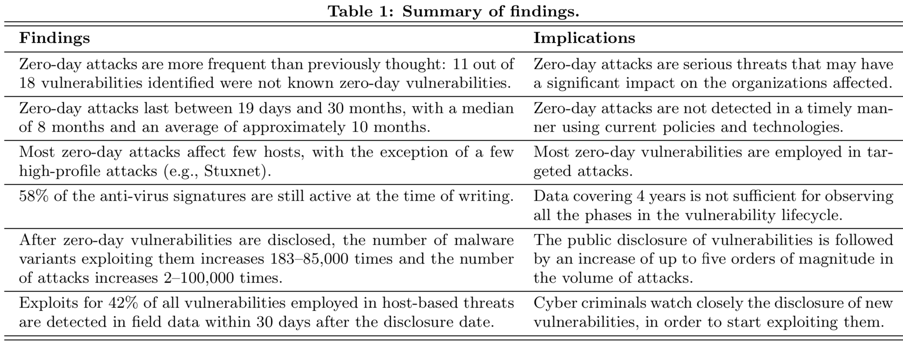
\includegraphics[width=\textwidth]{images/Disclosure_Research_Findings.PNG}
    \caption{Symantec's disclosure research findings} \label{fig:disclosure_research_findings}
\end{figure}

From Symantec's results, we conclude the following:

\begin{itemize}
    \item Zero days exist
    \item Usually zero days are targeted, and not highly used so that they would
    remain secret.
    \item Disclosure is terrible for security; after a patch is released,
    attackers use it to find the vulnerabilities and exploit them. Attackers go
    through public responsible disclosure and attack even before a patch is
    released. Between the point where the disclosure was made publicly and the
    patch deployment was completed, the scale of attacks rose by 5 orders of
    magnitude, making public disclosure a bad idea.
\end{itemize}

\paragraph{Responsible disclosure.} There is a government operated website
called CVE – Common Vulnerabilities and Exposures. Disclosure could be performed
by uploading a vulnerability to the site such that only the owner of the
software can see it, and publish the details only when a patch is released
(between points $t_p$ and $t_a$ in \cref{fig:vulnerability_timeline}), to avoid
the window when the vulnerability is public and unpatched (between $t_0$ and
$t_p$ in \cref{fig:vulnerability_timeline}). Microsoft called this practice of
disclosing privately Coordinated Vulnerability Disclosure, and claim it
significantly reduces the amount of exploits on new vulnerabilities\cite{CVD}.

Google introduced a system\cite{googleDisclosure} where the vulnerability remains private for 90 days,
after which it goes public, with or without a patch. The strict deadline is
meant to make sure the vulnerable vendor does not dismiss fixing the bug due to
it being unknown, and thus security is improved.

Over the years using machine learning with CVEs was used for detecting and classifing vulnerabilities in code\cite{mokhov2010use}, 
as well as making automatic predictions for unseen vulnerabilities\cite{edkrantz2015predicting}.

On the other hand, CVEs can be used to find unpatched exploits – for example, there was a bug in Linux
which hasn't yet gone public, but someone needed to commit the changes, which
contained the CVE-ID. Thus hackers could see the fix and exploit the
vulnerability before a patch was posted.
